%\documentclass[12pt]{article}
\documentclass[12pt,landscape]{article}


%packages
%\usepackage{latexsym}
\usepackage{graphicx}
\usepackage{color}
\usepackage{amsmath}
\usepackage{dsfont}
\usepackage{placeins}
\usepackage{amssymb}
\usepackage{wasysym}
\usepackage{abstract}
\usepackage{hyperref}
\usepackage{etoolbox}
\usepackage{datetime}
\usepackage{xcolor}
\usepackage{alphalph}
\settimeformat{ampmtime}

%\usepackage{pstricks,pst-node,pst-tree}

%\usepackage{algpseudocode}
%\usepackage{amsthm}
%\usepackage{hyperref}
%\usepackage{mathrsfs}
%\usepackage{amsfonts}
%\usepackage{bbding}
%\usepackage{listings}
%\usepackage{appendix}
\usepackage[margin=1in]{geometry}
%\geometry{papersize={8.5in,11in},total={6.5in,9in}}
%\usepackage{cancel}
%\usepackage{algorithmic, algorithm}

\makeatletter
\def\maxwidth{ %
  \ifdim\Gin@nat@width>\linewidth
    \linewidth
  \else
    \Gin@nat@width
  \fi
}
\makeatother

\definecolor{fgcolor}{rgb}{0.345, 0.345, 0.345}
\newcommand{\hlnum}[1]{\textcolor[rgb]{0.686,0.059,0.569}{#1}}%
\newcommand{\hlstr}[1]{\textcolor[rgb]{0.192,0.494,0.8}{#1}}%
\newcommand{\hlcom}[1]{\textcolor[rgb]{0.678,0.584,0.686}{\textit{#1}}}%
\newcommand{\hlopt}[1]{\textcolor[rgb]{0,0,0}{#1}}%
\newcommand{\hlstd}[1]{\textcolor[rgb]{0.345,0.345,0.345}{#1}}%
\newcommand{\hlkwa}[1]{\textcolor[rgb]{0.161,0.373,0.58}{\textbf{#1}}}%
\newcommand{\hlkwb}[1]{\textcolor[rgb]{0.69,0.353,0.396}{#1}}%
\newcommand{\hlkwc}[1]{\textcolor[rgb]{0.333,0.667,0.333}{#1}}%
\newcommand{\hlkwd}[1]{\textcolor[rgb]{0.737,0.353,0.396}{\textbf{#1}}}%

\usepackage{framed}
\makeatletter
\newenvironment{kframe}{%
 \def\at@end@of@kframe{}%
 \ifinner\ifhmode%
  \def\at@end@of@kframe{\end{minipage}}%
  \begin{minipage}{\columnwidth}%
 \fi\fi%
 \def\FrameCommand##1{\hskip\@totalleftmargin \hskip-\fboxsep
 \colorbox{shadecolor}{##1}\hskip-\fboxsep
     % There is no \\@totalrightmargin, so:
     \hskip-\linewidth \hskip-\@totalleftmargin \hskip\columnwidth}%
 \MakeFramed {\advance\hsize-\width
   \@totalleftmargin\z@ \linewidth\hsize
   \@setminipage}}%
 {\par\unskip\endMakeFramed%
 \at@end@of@kframe}
\makeatother

\definecolor{shadecolor}{rgb}{.77, .77, .77}
\definecolor{messagecolor}{rgb}{0, 0, 0}
\definecolor{warningcolor}{rgb}{1, 0, 1}
\definecolor{errorcolor}{rgb}{1, 0, 0}
\newenvironment{knitrout}{}{} % an empty environment to be redefined in TeX

\usepackage{alltt}
\usepackage[T1]{fontenc}

\newcommand{\qu}[1]{``#1''}
\newcounter{probnum}
\setcounter{probnum}{1}

%create definition to allow local margin changes
\def\changemargin#1#2{\list{}{\rightmargin#2\leftmargin#1}\item[]}
\let\endchangemargin=\endlist 

%allow equations to span multiple pages
\allowdisplaybreaks

%define colors and color typesetting conveniences
\definecolor{gray}{rgb}{0.5,0.5,0.5}
\definecolor{black}{rgb}{0,0,0}
\definecolor{white}{rgb}{1,1,1}
\definecolor{blue}{rgb}{0.5,0.5,1}
\newcommand{\inblue}[1]{\color{blue}#1 \color{black}}
\definecolor{green}{rgb}{0.133,0.545,0.133}
\newcommand{\ingreen}[1]{\color{green}#1 \color{black}}
\definecolor{yellow}{rgb}{1,1,0}
\newcommand{\inyellow}[1]{\color{yellow}#1 \color{black}}
\definecolor{orange}{rgb}{0.9,0.649,0}
\newcommand{\inorange}[1]{\color{orange}#1 \color{black}}
\definecolor{red}{rgb}{1,0.133,0.133}
\newcommand{\inred}[1]{\color{red}#1 \color{black}}
\definecolor{purple}{rgb}{0.58,0,0.827}
\newcommand{\inpurple}[1]{\color{purple}#1 \color{black}}
\definecolor{backgcode}{rgb}{0.97,0.97,0.8}
\definecolor{Brown}{cmyk}{0,0.81,1,0.60}
\definecolor{OliveGreen}{cmyk}{0.64,0,0.95,0.40}
\definecolor{CadetBlue}{cmyk}{0.62,0.57,0.23,0}

%define new math operators
\DeclareMathOperator*{\argmax}{arg\,max~}
\DeclareMathOperator*{\argmin}{arg\,min~}
\DeclareMathOperator*{\argsup}{arg\,sup~}
\DeclareMathOperator*{\arginf}{arg\,inf~}
\DeclareMathOperator*{\convolution}{\text{\Huge{$\ast$}}}
\newcommand{\infconv}[2]{\convolution^\infty_{#1 = 1} #2}
%true functions

%%%% GENERAL SHORTCUTS

%shortcuts for pure typesetting conveniences
\newcommand{\bv}[1]{\boldsymbol{#1}}

%shortcuts for compound constants
\newcommand{\BetaDistrConst}{\dfrac{\Gamma(\alpha + \beta)}{\Gamma(\alpha)\Gamma(\beta)}}
\newcommand{\NormDistrConst}{\dfrac{1}{\sqrt{2\pi\sigma^2}}}

%shortcuts for conventional symbols
\newcommand{\tsq}{\tau^2}
\newcommand{\tsqh}{\hat{\tau}^2}
\newcommand{\sigsq}{\sigma^2}
\newcommand{\sigsqsq}{\parens{\sigma^2}^2}
\newcommand{\sigsqovern}{\dfrac{\sigsq}{n}}
\newcommand{\tausq}{\tau^2}
\newcommand{\tausqalpha}{\tau^2_\alpha}
\newcommand{\tausqbeta}{\tau^2_\beta}
\newcommand{\tausqsigma}{\tau^2_\sigma}
\newcommand{\betasq}{\beta^2}
\newcommand{\sigsqvec}{\bv{\sigma}^2}
\newcommand{\sigsqhat}{\hat{\sigma}^2}
\newcommand{\sigsqhatmlebayes}{\sigsqhat_{\text{Bayes, MLE}}}
\newcommand{\sigsqhatmle}[1]{\sigsqhat_{#1, \text{MLE}}}
\newcommand{\bSigma}{\bv{\Sigma}}
\newcommand{\bSigmainv}{\bSigma^{-1}}
\newcommand{\thetavec}{\bv{\theta}}
\newcommand{\thetahat}{\hat{\theta}}
\newcommand{\thetahatmle}{\hat{\theta}_{\mathrm{MLE}}}
\newcommand{\thetavechatmle}{\hat{\thetavec}_{\mathrm{MLE}}}
\newcommand{\muhat}{\hat{\mu}}
\newcommand{\musq}{\mu^2}
\newcommand{\muvec}{\bv{\mu}}
\newcommand{\muhatmle}{\muhat_{\text{MLE}}}
\newcommand{\lambdahat}{\hat{\lambda}}
\newcommand{\lambdahatmle}{\lambdahat_{\text{MLE}}}
\newcommand{\etavec}{\bv{\eta}}
\newcommand{\alphavec}{\bv{\alpha}}
\newcommand{\minimaxdec}{\delta^*_{\mathrm{mm}}}
\newcommand{\ybar}{\bar{y}}
\newcommand{\xbar}{\bar{x}}
\newcommand{\Xbar}{\bar{X}}
\newcommand{\phat}{\hat{p}}
\newcommand{\Phat}{\hat{P}}
\newcommand{\Zbar}{\bar{Z}}
\newcommand{\iid}{~{\buildrel iid \over \sim}~}
\newcommand{\inddist}{~{\buildrel ind \over \sim}~}
\newcommand{\approxdist}{~{\buildrel approx \over \sim}~}
\newcommand{\equalsindist}{~{\buildrel d \over =}~}
\newcommand{\loglik}[1]{\ell\parens{#1}}
\newcommand{\thetahatkminone}{\thetahat^{(k-1)}}
\newcommand{\thetahatkplusone}{\thetahat^{(k+1)}}
\newcommand{\thetahatk}{\thetahat^{(k)}}
\newcommand{\half}{\frac{1}{2}}
\newcommand{\third}{\frac{1}{3}}
\newcommand{\twothirds}{\frac{2}{3}}
\newcommand{\fourth}{\frac{1}{4}}
\newcommand{\fifth}{\frac{1}{5}}
\newcommand{\sixth}{\frac{1}{6}}

%shortcuts for vector and matrix notation
\newcommand{\A}{\bv{A}}
\newcommand{\At}{\A^T}
\newcommand{\Ainv}{\inverse{\A}}
\newcommand{\B}{\bv{B}}
\newcommand{\K}{\bv{K}}
\newcommand{\Kt}{\K^T}
\newcommand{\Kinv}{\inverse{K}}
\newcommand{\Kinvt}{(\Kinv)^T}
\newcommand{\M}{\bv{M}}
\newcommand{\Bt}{\B^T}
\newcommand{\Q}{\bv{Q}}
\newcommand{\Qt}{\Q^T}
\newcommand{\R}{\bv{R}}
\newcommand{\Rt}{\R^T}
\newcommand{\Z}{\bv{Z}}
\newcommand{\X}{\bv{X}}
\renewcommand{\H}{\bv{H}}
\newcommand{\Xsub}{\X_{\text{(sub)}}}
\newcommand{\Xsubadj}{\X_{\text{(sub,adj)}}}
\newcommand{\I}{\bv{I}}
\newcommand{\Y}{\bv{Y}}
\newcommand{\sigsqI}{\sigsq\I}
\renewcommand{\P}{\bv{P}}
\newcommand{\Psub}{\P_{\text{(sub)}}}
\newcommand{\Pt}{\P^T}
\newcommand{\Pii}{P_{ii}}
\newcommand{\Pij}{P_{ij}}
\newcommand{\IminP}{(\I-\P)}
\newcommand{\Xt}{\bv{X}^T}
\newcommand{\XtX}{\Xt\X}
\newcommand{\XtXinv}{\parens{\Xt\X}^{-1}}
\newcommand{\XtXinvXt}{\XtXinv\Xt}
\newcommand{\XXtXinvXt}{\X\XtXinvXt}
\newcommand{\x}{\bv{x}}
\renewcommand{\b}{\bv{b}}
\newcommand{\onevec}{\bv{1}}
\newcommand{\oneton}{1, \ldots, n}
\newcommand{\yoneton}{y_1, \ldots, y_n}
\newcommand{\yonetonorder}{y_{(1)}, \ldots, y_{(n)}}
\newcommand{\Yoneton}{Y_1, \ldots, Y_n}
\newcommand{\iinoneton}{i \in \braces{\oneton}}
\newcommand{\onetom}{1, \ldots, m}
\newcommand{\jinonetom}{j \in \braces{\onetom}}
\newcommand{\xoneton}{x_1, \ldots, x_n}
\newcommand{\Xoneton}{X_1, \ldots, X_n}
\newcommand{\xt}{\x^T}
\newcommand{\y}{\bv{y}}
\newcommand{\yt}{\y^T}
\renewcommand{\c}{\bv{c}}
\newcommand{\ct}{\c^T}
\newcommand{\tstar}{\bv{t}^*}
\renewcommand{\u}{\bv{u}}
\renewcommand{\v}{\bv{v}}
\renewcommand{\a}{\bv{a}}
\newcommand{\s}{\bv{s}}
\newcommand{\yadj}{\y_{\text{(adj)}}}
\newcommand{\xjadj}{\x_{j\text{(adj)}}}
\newcommand{\xjadjM}{\x_{j \perp M}}
\newcommand{\yhat}{\hat{\y}}
\newcommand{\yhatsub}{\yhat_{\text{(sub)}}}
\newcommand{\yhatstar}{\yhat^*}
\newcommand{\yhatstarnew}{\yhatstar_{\text{new}}}
\newcommand{\z}{\bv{z}}
\newcommand{\zt}{\z^T}
\newcommand{\bb}{\bv{b}}
\newcommand{\bbt}{\bb^T}
\newcommand{\bbeta}{\bv{\beta}}
\newcommand{\beps}{\bv{\epsilon}}
\newcommand{\bepst}{\beps^T}
\newcommand{\e}{\bv{e}}
\newcommand{\Mofy}{\M(\y)}
\newcommand{\KofAlpha}{K(\alpha)}
\newcommand{\ellset}{\mathcal{L}}
\newcommand{\oneminalph}{1-\alpha}
\newcommand{\SSE}{\text{SSE}}
\newcommand{\SSEsub}{\text{SSE}_{\text{(sub)}}}
\newcommand{\MSE}{\text{MSE}}
\newcommand{\RMSE}{\text{RMSE}}
\newcommand{\SSR}{\text{SSR}}
\newcommand{\SST}{\text{SST}}
\newcommand{\JSest}{\delta_{\text{JS}}(\x)}
\newcommand{\Bayesest}{\delta_{\text{Bayes}}(\x)}
\newcommand{\EmpBayesest}{\delta_{\text{EmpBayes}}(\x)}
\newcommand{\BLUPest}{\delta_{\text{BLUP}}}
\newcommand{\MLEest}[1]{\hat{#1}_{\text{MLE}}}

%shortcuts for Linear Algebra stuff (i.e. vectors and matrices)
\newcommand{\twovec}[2]{\bracks{\begin{array}{c} #1 \\ #2 \end{array}}}
\newcommand{\threevec}[3]{\bracks{\begin{array}{c} #1 \\ #2 \\ #3 \end{array}}}
\newcommand{\fivevec}[5]{\bracks{\begin{array}{c} #1 \\ #2 \\ #3 \\ #4 \\ #5 \end{array}}}
\newcommand{\twobytwomat}[4]{\bracks{\begin{array}{cc} #1 & #2 \\ #3 & #4 \end{array}}}
\newcommand{\threebytwomat}[6]{\bracks{\begin{array}{cc} #1 & #2 \\ #3 & #4 \\ #5 & #6 \end{array}}}

%shortcuts for conventional compound symbols
\newcommand{\thetainthetas}{\theta \in \Theta}
\newcommand{\reals}{\mathbb{R}}
\newcommand{\complexes}{\mathbb{C}}
\newcommand{\rationals}{\mathbb{Q}}
\newcommand{\integers}{\mathbb{Z}}
\newcommand{\naturals}{\mathbb{N}}
\newcommand{\forallninN}{~~\forall n \in \naturals}
\newcommand{\forallxinN}[1]{~~\forall #1 \in \reals}
\newcommand{\matrixdims}[2]{\in \reals^{\,#1 \times #2}}
\newcommand{\inRn}[1]{\in \reals^{\,#1}}
\newcommand{\mathimplies}{\quad\Rightarrow\quad}
\newcommand{\mathlogicequiv}{\quad\Leftrightarrow\quad}
\newcommand{\eqncomment}[1]{\quad \text{(#1)}}
\newcommand{\limitn}{\lim_{n \rightarrow \infty}}
\newcommand{\limitN}{\lim_{N \rightarrow \infty}}
\newcommand{\limitd}{\lim_{d \rightarrow \infty}}
\newcommand{\limitt}{\lim_{t \rightarrow \infty}}
\newcommand{\limitsupn}{\limsup_{n \rightarrow \infty}~}
\newcommand{\limitinfn}{\liminf_{n \rightarrow \infty}~}
\newcommand{\limitk}{\lim_{k \rightarrow \infty}}
\newcommand{\limsupn}{\limsup_{n \rightarrow \infty}}
\newcommand{\limsupk}{\limsup_{k \rightarrow \infty}}
\newcommand{\floor}[1]{\left\lfloor #1 \right\rfloor}
\newcommand{\ceil}[1]{\left\lceil #1 \right\rceil}

%shortcuts for environments
\newcommand{\beqn}{\vspace{-0.25cm}\begin{eqnarray*}}
\newcommand{\eeqn}{\end{eqnarray*}}
\newcommand{\bneqn}{\vspace{-0.25cm}\begin{eqnarray}}
\newcommand{\eneqn}{\end{eqnarray}}

%shortcuts for mini environments
\newcommand{\parens}[1]{\left(#1\right)}
\newcommand{\squared}[1]{\parens{#1}^2}
\newcommand{\tothepow}[2]{\parens{#1}^{#2}}
\newcommand{\prob}[1]{\mathbb{P}\parens{#1}}
\newcommand{\cprob}[2]{\prob{#1~|~#2}}
\newcommand{\littleo}[1]{o\parens{#1}}
\newcommand{\bigo}[1]{O\parens{#1}}
\newcommand{\Lp}[1]{\mathbb{L}^{#1}}
\renewcommand{\arcsin}[1]{\text{arcsin}\parens{#1}}
\newcommand{\prodonen}[2]{\bracks{\prod_{#1=1}^n #2}}
\newcommand{\mysum}[4]{\sum_{#1=#2}^{#3} #4}
\newcommand{\sumonen}[2]{\sum_{#1=1}^n #2}
\newcommand{\infsum}[2]{\sum_{#1=1}^\infty #2}
\newcommand{\infprod}[2]{\prod_{#1=1}^\infty #2}
\newcommand{\infunion}[2]{\bigcup_{#1=1}^\infty #2}
\newcommand{\infinter}[2]{\bigcap_{#1=1}^\infty #2}
\newcommand{\infintegral}[2]{\int^\infty_{-\infty} #2 ~\text{d}#1}
\newcommand{\supthetas}[1]{\sup_{\thetainthetas}\braces{#1}}
\newcommand{\bracks}[1]{\left[#1\right]}
\newcommand{\braces}[1]{\left\{#1\right\}}
\newcommand{\set}[1]{\left\{#1\right\}}
\newcommand{\abss}[1]{\left|#1\right|}
\newcommand{\norm}[1]{\left|\left|#1\right|\right|}
\newcommand{\normsq}[1]{\norm{#1}^2}
\newcommand{\inverse}[1]{\parens{#1}^{-1}}
\newcommand{\rowof}[2]{\parens{#1}_{#2\cdot}}

%shortcuts for functionals
\newcommand{\realcomp}[1]{\text{Re}\bracks{#1}}
\newcommand{\imagcomp}[1]{\text{Im}\bracks{#1}}
\newcommand{\range}[1]{\text{range}\bracks{#1}}
\newcommand{\colsp}[1]{\text{colsp}\bracks{#1}}
\newcommand{\rowsp}[1]{\text{rowsp}\bracks{#1}}
\newcommand{\tr}[1]{\text{tr}\bracks{#1}}
\newcommand{\rank}[1]{\text{rank}\bracks{#1}}
\newcommand{\proj}[2]{\text{Proj}_{#1}\bracks{#2}}
\newcommand{\projcolspX}[1]{\text{Proj}_{\colsp{\X}}\bracks{#1}}
\newcommand{\median}[1]{\text{median}\bracks{#1}}
\newcommand{\mean}[1]{\text{mean}\bracks{#1}}
\newcommand{\dime}[1]{\text{dim}\bracks{#1}}
\renewcommand{\det}[1]{\text{det}\bracks{#1}}
\newcommand{\expe}[1]{\mathbb{E}\bracks{#1}}
\newcommand{\expeabs}[1]{\expe{\abss{#1}}}
\newcommand{\expesub}[2]{\mathbb{E}_{#1}\bracks{#2}}
\newcommand{\indic}[1]{\mathds{1}_{#1}}
\newcommand{\var}[1]{\mathbb{V}\text{ar}\bracks{#1}}
\newcommand{\cov}[2]{\mathbb{C}\text{ov}\bracks{#1, #2}}
\newcommand{\corr}[2]{\text{Corr}\bracks{#1, #2}}
\newcommand{\se}[1]{\mathbb{S}\text{E}\bracks{#1}}
\newcommand{\seest}[1]{\hat{\mathbb{S}\text{E}}\bracks{#1}}
\newcommand{\bias}[1]{\text{Bias}\bracks{#1}}
\newcommand{\derivop}[2]{\dfrac{\text{d}}{\text{d} #1}\bracks{#2}}
\newcommand{\partialop}[2]{\dfrac{\partial}{\partial #1}\bracks{#2}}
\newcommand{\secpartialop}[2]{\dfrac{\partial^2}{\partial #1^2}\bracks{#2}}
\newcommand{\mixpartialop}[3]{\dfrac{\partial^2}{\partial #1 \partial #2}\bracks{#3}}

%shortcuts for functions
\renewcommand{\exp}[1]{\mathrm{exp}\parens{#1}}
\renewcommand{\cos}[1]{\text{cos}\parens{#1}}
\renewcommand{\sin}[1]{\text{sin}\parens{#1}}
\newcommand{\sign}[1]{\text{sign}\parens{#1}}
\newcommand{\are}[1]{\mathrm{ARE}\parens{#1}}
\newcommand{\natlog}[1]{\ln\parens{#1}}
\newcommand{\oneover}[1]{\frac{1}{#1}}
\newcommand{\overtwo}[1]{\frac{#1}{2}}
\newcommand{\overn}[1]{\frac{#1}{n}}
\newcommand{\oneoversqrt}[1]{\oneover{\sqrt{#1}}}
\newcommand{\sqd}[1]{\parens{#1}^2}
\newcommand{\loss}[1]{\ell\parens{\theta, #1}}
\newcommand{\losstwo}[2]{\ell\parens{#1, #2}}
\newcommand{\cf}{\phi(t)}

%English language specific shortcuts
\newcommand{\ie}{\textit{i.e.} }
\newcommand{\AKA}{\textit{AKA} }
\renewcommand{\iff}{\textit{iff}}
\newcommand{\eg}{\textit{e.g.} }
\newcommand{\st}{\textit{s.t.} }
\newcommand{\wrt}{\textit{w.r.t.} }
\newcommand{\mathst}{~~\text{\st}~~}
\newcommand{\mathand}{~~\text{and}~~}
\newcommand{\ala}{\textit{a la} }
\newcommand{\ppp}{posterior predictive p-value}
\newcommand{\dd}{dataset-to-dataset}

%shortcuts for distribution titles
\newcommand{\logistic}[2]{\mathrm{Logistic}\parens{#1,\,#2}}
\newcommand{\bernoulli}[1]{\mathrm{Bernoulli}\parens{#1}}
\newcommand{\betanot}[2]{\mathrm{Beta}\parens{#1,\,#2}}
\newcommand{\stdbetanot}{\betanot{\alpha}{\beta}}
\newcommand{\multnormnot}[3]{\mathcal{N}_{#1}\parens{#2,\,#3}}
\newcommand{\normnot}[2]{\mathcal{N}\parens{#1,\,#2}}
\newcommand{\classicnormnot}{\normnot{\mu}{\sigsq}}
\newcommand{\stdnormnot}{\normnot{0}{1}}
\newcommand{\uniformdiscrete}[1]{\mathrm{Uniform}\parens{\braces{#1}}}
\newcommand{\uniform}[2]{\mathrm{U}\parens{#1,\,#2}}
\newcommand{\stduniform}{\uniform{0}{1}}
\newcommand{\geometric}[1]{\mathrm{Geometric}\parens{#1}}
\newcommand{\hypergeometric}[3]{\mathrm{Hypergeometric}\parens{#1,\,#2,\,#3}}
\newcommand{\exponential}[1]{\mathrm{Exp}\parens{#1}}
\newcommand{\gammadist}[2]{\mathrm{Gamma}\parens{#1, #2}}
\newcommand{\poisson}[1]{\mathrm{Poisson}\parens{#1}}
\newcommand{\binomial}[2]{\mathrm{Binomial}\parens{#1,\,#2}}
\newcommand{\negbin}[2]{\mathrm{NegBin}\parens{#1,\,#2}}
\newcommand{\rayleigh}[1]{\mathrm{Rayleigh}\parens{#1}}
\newcommand{\multinomial}[2]{\mathrm{Multinomial}\parens{#1,\,#2}}
\newcommand{\gammanot}[2]{\mathrm{Gamma}\parens{#1,\,#2}}
\newcommand{\cauchynot}[2]{\text{Cauchy}\parens{#1,\,#2}}
\newcommand{\invchisqnot}[1]{\text{Inv}\chisq{#1}}
\newcommand{\invscaledchisqnot}[2]{\text{ScaledInv}\ncchisq{#1}{#2}}
\newcommand{\invgammanot}[2]{\text{InvGamma}\parens{#1,\,#2}}
\newcommand{\chisq}[1]{\chi^2_{#1}}
\newcommand{\ncchisq}[2]{\chi^2_{#1}\parens{#2}}
\newcommand{\ncF}[3]{F_{#1,#2}\parens{#3}}

%shortcuts for PDF's of common distributions
\newcommand{\logisticpdf}[3]{\oneover{#3}\dfrac{\exp{-\dfrac{#1 - #2}{#3}}}{\parens{1+\exp{-\dfrac{#1 - #2}{#3}}}^2}}
\newcommand{\betapdf}[3]{\dfrac{\Gamma(#2 + #3)}{\Gamma(#2)\Gamma(#3)}#1^{#2-1} (1-#1)^{#3-1}}
\newcommand{\normpdf}[3]{\frac{1}{\sqrt{2\pi#3}}\exp{-\frac{1}{2#3}(#1 - #2)^2}}
\newcommand{\normpdfvarone}[2]{\dfrac{1}{\sqrt{2\pi}}e^{-\half(#1 - #2)^2}}
\newcommand{\chisqpdf}[2]{\dfrac{1}{2^{#2/2}\Gamma(#2/2)}\; {#1}^{#2/2-1} e^{-#1/2}}
\newcommand{\invchisqpdf}[2]{\dfrac{2^{-\overtwo{#1}}}{\Gamma(#2/2)}\,{#1}^{-\overtwo{#2}-1}  e^{-\oneover{2 #1}}}
\newcommand{\exponentialpdf}[2]{#2\exp{-#2#1}}
\newcommand{\poissonpdf}[2]{\dfrac{e^{-#1} #1^{#2}}{#2!}}
\newcommand{\binomialpdf}[3]{\binom{#2}{#1}#3^{#1}(1-#3)^{#2-#1}}
\newcommand{\rayleighpdf}[2]{\dfrac{#1}{#2^2}\exp{-\dfrac{#1^2}{2 #2^2}}}
\newcommand{\gammapdf}[3]{\dfrac{#3^#2}{\Gamma\parens{#2}}#1^{#2-1}\exp{-#3 #1}}
\newcommand{\cauchypdf}[3]{\oneover{\pi} \dfrac{#3}{\parens{#1-#2}^2 + #3^2}}
\newcommand{\Gammaf}[1]{\Gamma\parens{#1}}

%shortcuts for miscellaneous typesetting conveniences
\newcommand{\notesref}[1]{\marginpar{\color{gray}\tt #1\color{black}}}

%%%% DOMAIN-SPECIFIC SHORTCUTS

%Real analysis related shortcuts
\newcommand{\zeroonecl}{\bracks{0,1}}
\newcommand{\forallepsgrzero}{\forall \epsilon > 0~~}
\newcommand{\lessthaneps}{< \epsilon}
\newcommand{\fraccomp}[1]{\text{frac}\bracks{#1}}

%Bayesian related shortcuts
\newcommand{\yrep}{y^{\text{rep}}}
\newcommand{\yrepisq}{(\yrep_i)^2}
\newcommand{\yrepvec}{\bv{y}^{\text{rep}}}


%Probability shortcuts
\newcommand{\SigField}{\mathcal{F}}
\newcommand{\ProbMap}{\mathcal{P}}
\newcommand{\probtrinity}{\parens{\Omega, \SigField, \ProbMap}}
\newcommand{\convp}{~{\buildrel p \over \rightarrow}~}
\newcommand{\convLp}[1]{~{\buildrel \Lp{#1} \over \rightarrow}~}
\newcommand{\nconvp}{~{\buildrel p \over \nrightarrow}~}
\newcommand{\convae}{~{\buildrel a.e. \over \longrightarrow}~}
\newcommand{\convau}{~{\buildrel a.u. \over \longrightarrow}~}
\newcommand{\nconvau}{~{\buildrel a.u. \over \nrightarrow}~}
\newcommand{\nconvae}{~{\buildrel a.e. \over \nrightarrow}~}
\newcommand{\convd}{~{\buildrel \mathcal{D} \over \rightarrow}~}
\newcommand{\nconvd}{~{\buildrel \mathcal{D} \over \nrightarrow}~}
\newcommand{\withprob}{~~\text{w.p.}~~}
\newcommand{\io}{~~\text{i.o.}}

\newcommand{\Acl}{\bar{A}}
\newcommand{\ENcl}{\bar{E}_N}
\newcommand{\diam}[1]{\text{diam}\parens{#1}}

\newcommand{\taua}{\tau_a}

\newcommand{\myint}[4]{\int_{#2}^{#3} #4 \,\text{d}#1}
\newcommand{\laplacet}[1]{\mathscr{L}\bracks{#1}}
\newcommand{\laplaceinvt}[1]{\mathscr{L}^{-1}\bracks{#1}}
\renewcommand{\min}[1]{\text{min}\braces{#1}}
\renewcommand{\max}[1]{\text{max}\braces{#1}}

\newcommand{\Vbar}[1]{\bar{V}\parens{#1}}
\newcommand{\expnegrtau}{\exp{-r\tau}}

%%% problem typesetting
\definecolor{darkgrey}{rgb}{0.10,0.10,0.9}

\newcommand{\problem}[1]{\noindent \colorbox{black}{{\color{yellow} \large{\textsf{\textbf{Problem \arabic{probnum}}}}~}} \addtocounter{probnum}{1} \vspace{0.2cm} \\ \iftoggle{professormode}{}{\color{darkgrey}} #1}

\newcommand{\easysubproblem}[1]{\ingreen{\item} \iftoggle{professormode}{}{\color{darkgrey}} [easy] #1 \color{black} }
\newcommand{\intermediatesubproblem}[1]{\inorange{\item} \iftoggle{professormode}{}{\color{darkgrey}} [harder] #1 \color{black} }
\newcommand{\hardsubproblem}[1]{\inred{\item} \iftoggle{professormode}{}{\color{darkgrey}} [difficult] #1 \color{black} }
\newcommand{\extracreditsubproblem}[1]{\inpurple{\item} \iftoggle{professormode}{}{\color{darkgrey}} [E.C.] #1 \color{black} }


\newcommand{\spc}[1]{\iftoggle{professormode}{\\ \vspace{#1cm}}{\\ \vspace{-0.3cm}}}

\makeatletter
\newalphalph{\alphmult}[mult]{\@alph}{26}
\renewcommand{\labelenumi}{(\alphmult{\value{enumi}})}

\newcommand{\support}[1]{\text{Supp}\bracks{#1}}
\newcommand{\mode}[1]{\text{Mode}\bracks{#1}}
\newcommand{\IQR}[1]{\text{IQR}\bracks{#1}}
\newcommand{\quantile}[2]{\text{Quantile}\bracks{#1,\,#2}}


\newcommand{\instr}{\small Your answer will consist of a lowercase string (e.g. \texttt{aebgd}) where the order of the letters does not matter. \normalsize}

\title{Math 342W / 650 Fall \the\year{} \\ Midterm Examination Two}
\author{Professor Adam Kapelner}

\date{Thursday, May 13, \the\year{}}

\begin{document}
\maketitle

%\noindent Full Name \line(1,0){410}

\thispagestyle{empty}

\section*{Code of Academic Integrity}

\footnotesize
Since the college is an academic community, its fundamental purpose is the pursuit of knowledge. Essential to the success of this educational mission is a commitment to the principles of academic integrity. Every member of the college community is responsible for upholding the highest standards of honesty at all times. Students, as members of the community, are also responsible for adhering to the principles and spirit of the following Code of Academic Integrity.

Activities that have the effect or intention of interfering with education, pursuit of knowledge, or fair evaluation of a student's performance are prohibited. Examples of such activities include but are not limited to the following definitions:

\paragraph{Cheating} Using or attempting to use unauthorized assistance, material, or study aids in examinations or other academic work or preventing, or attempting to prevent, another from using authorized assistance, material, or study aids. Example: using an unauthorized cheat sheet in a quiz or exam, altering a graded exam and resubmitting it for a better grade, etc.
\\

\noindent By taking this exam, you acknowledge and agree to uphold this Code of Academic Integrity. \\

%\begin{center}
%\line(1,0){250} ~~~ \line(1,0){100}\\
%~~~~~~~~~~~~~~~~~~~~~signature~~~~~~~~~~~~~~~~~~~~~~~~~~~~~~~~~~~~~~~~~~~~~ date
%\end{center}

\normalsize

\section*{Instructions}
This exam is 100 minutes (variable time per question) and closed-book. You are allowed \textbf{two} 8.5 $\times$ 11'' pages (front and back) of a \qu{cheat sheet}, blank scrap paper and a graphing calculator. Please read the questions carefully. No food is allowed, only drinks. %If the question reads \qu{compute,} this means the solution will be a number otherwise you can leave the answer in \textit{any} widely accepted mathematical notation which could be resolved to an exact or approximate number with the use of a computer. I advise you to skip problems marked \qu{[Extra Credit]} until you have finished the other questions on the exam, then loop back and plug in all the holes. I also advise you to use pencil. The exam is 100 points total plus extra credit. Partial credit will be granted for incomplete answers on most of the questions. \fbox{Box} in your final answers. Good luck!

\pagebreak


\problem\timedsection{11} Consider the following causal diagrams where all events have other causes that are not displayed. It is assumed that the timing of events is known and to scale. Assume you have a training set $\mathbb{D}$ with a large sample size $n$ with columns x, y, z (and w if included).


\vspace{-.3cm}
\begin{figure}[htp]
\centering
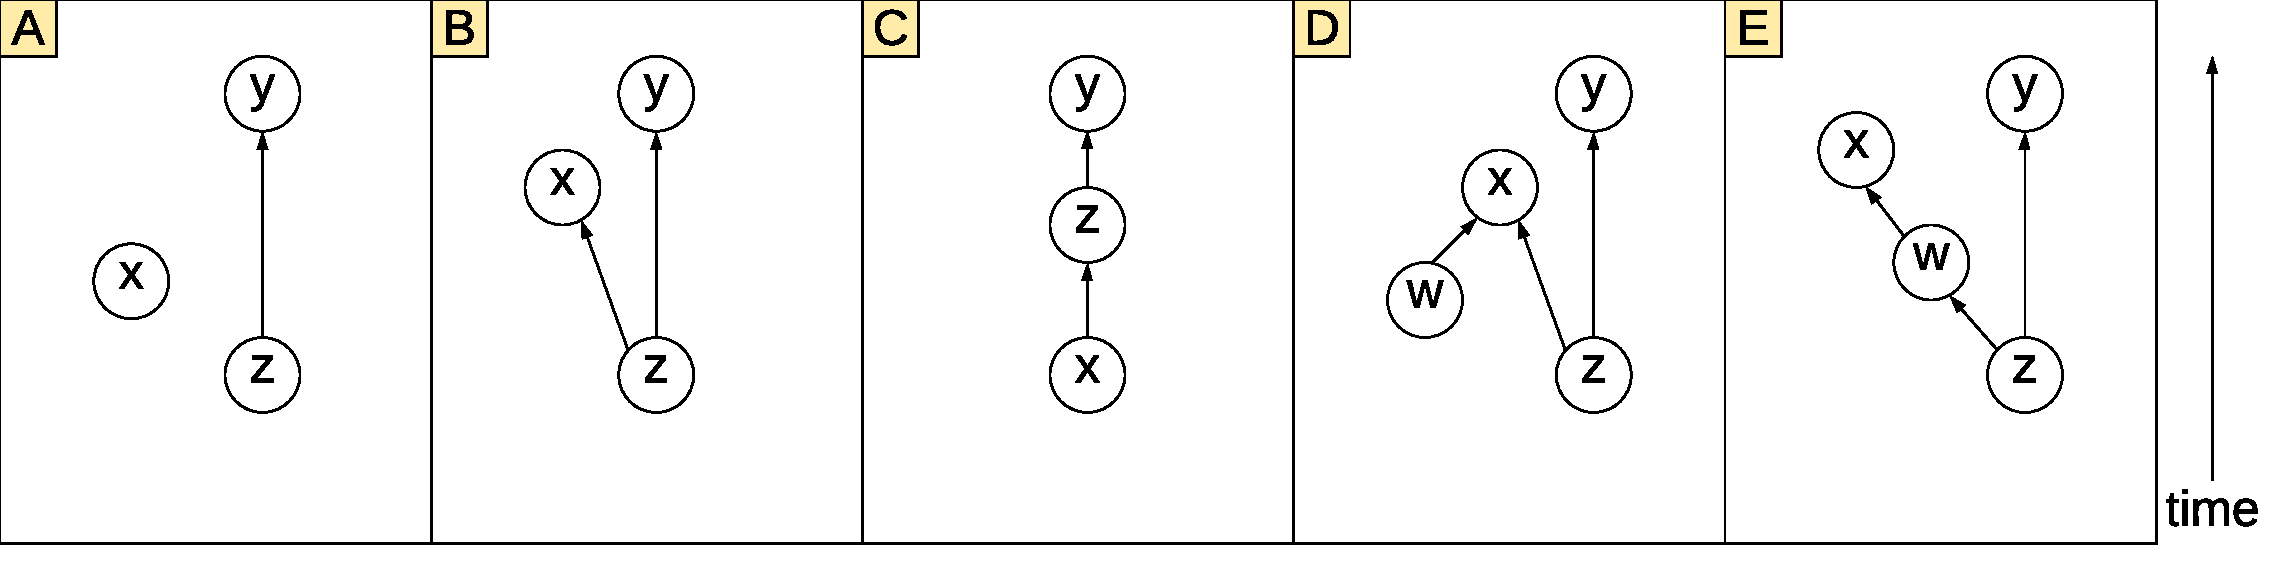
\includegraphics[width=7in]{basic_causal_diagrams}
\end{figure}

\vspace{-.4cm}

\vspace{-0.3cm}\benum\truefalsesubquestionwithpoints{11} 

\begin{enumerate}[(a)]
%\item In diagram A, x and z could be spuriously correlated.
%\item In diagram D, w and y could be spuriously correlated.
%\item In diagram E, w and y could be spuriously correlated.
%\item Assume the data generating process that $\mathbb{D}$ is sampled from is diagram A. When running the OLS model y $\sim$ x you find a strong correlation. This correlation is spurious.
\item Assume  diagram A is the data generating process that $\mathbb{D}$ is sampled from. When running the OLS model y $\sim$ x you find a strong correlation. In out-of-sample data there would likely be a near-zero correlation betweeen y and x.
\item In diagram A, z is a lurking variable when analyzing the causal effect of x on y.
\item In diagram B, z is a lurking variable when analyzing the causal effect of x on y.
\item In diagram D, w is a lurking variable when analyzing the causal effect of x on y.
\item In diagram E, w is a lurking variable when analyzing the causal effect of x on y.
\item In diagram C, x causes y (according to our in-class definition of causality).
\item In diagram B, an OLS model of y $\sim$ x demonstrates that x and y are correlated but this correlation disappears if you run an OLS model of y $\sim$ x + z
\item In diagram D, an OLS model of y $\sim$ x demonstrates that x and y are correlated but this correlation disappears if you run an OLS model of y $\sim$ x + w
\item In diagram D, x can be used to predict y better than $g_0$ (out of sample)
\item In diagram D, w can be used to predict y better than $g_0$ (out of sample)
\item In diagram E, an OLS model of y $\sim$ x demonstrates that x and y are correlated but this correlation disappears if you run an OLS model of y $\sim$ x + w

\end{enumerate}
\eenum\instr\pagebreak
%%%%%%%%%%%%%%%%%%%%%%%%%%%%%%%%%%%%%%%%%%%%%


%\problem\timedsection{7} \ingray{Consider the following causal diagrams where all events have other causes that are not displayed. It is assumed that the timing of events is known and to scale.} Assume now you have a training set $\mathbb{D}$ with a large sample size $n$ with columns x, y, z (and w if included).
%
%
%\begin{figure}[htp]
%\centering
%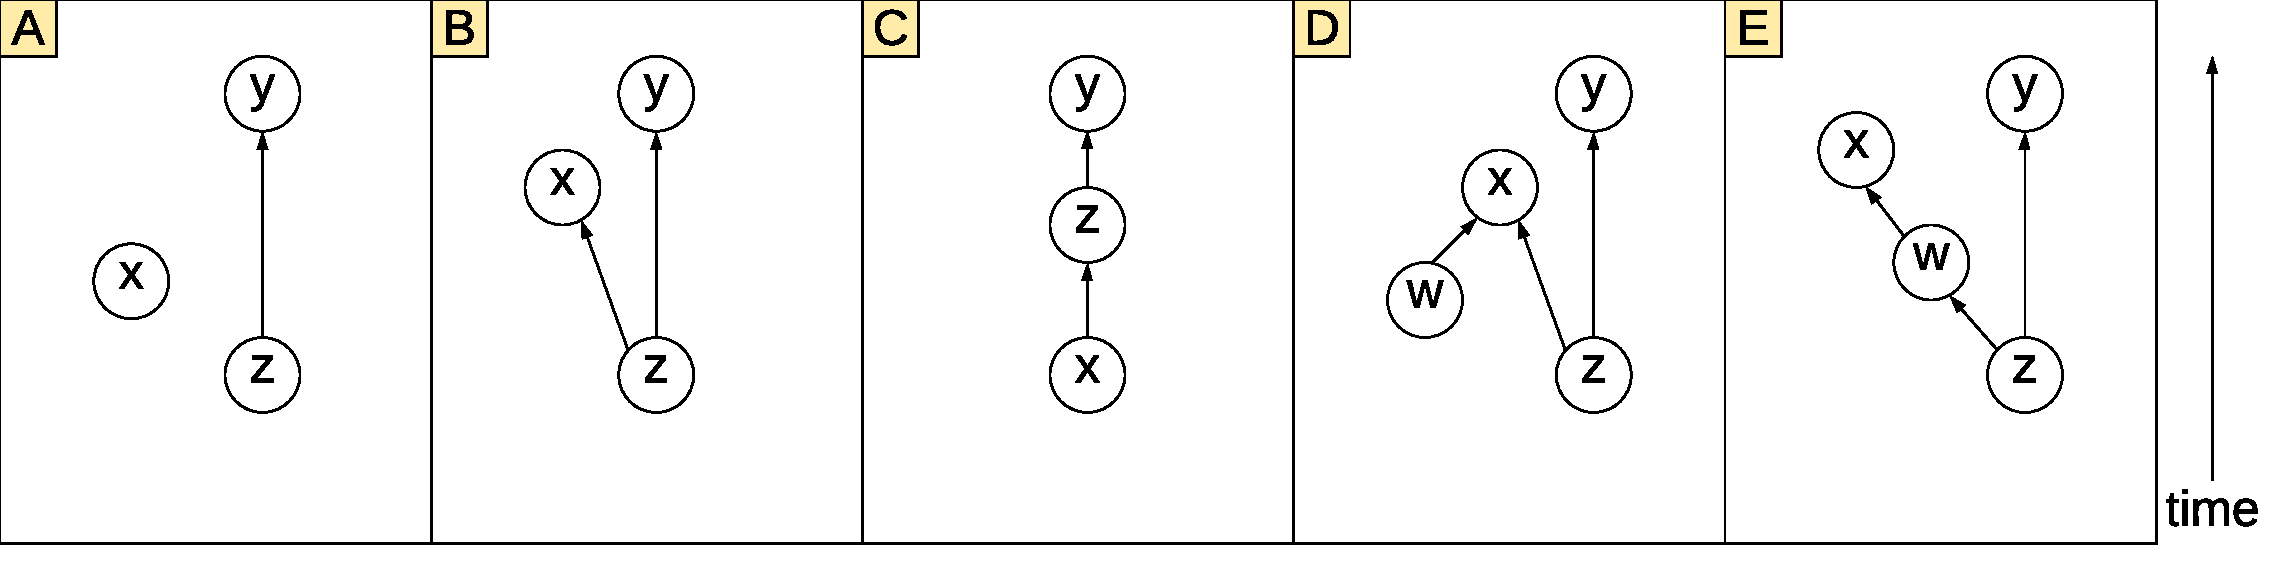
\includegraphics[width=7in]{basic_causal_diagrams}
%\end{figure}
%
%\vspace{-.5cm}
%
%\vspace{-0.2cm}\benum\truefalsesubquestionwithpoints{14} 
%
%\begin{enumerate}[(a)]
%\item Assume the data generating process that $\mathbb{D}$ is sampled from is diagram A. When running the OLS model y $\sim$ x you find a strong correlation. This correlation is spurious.
%\item Assume the data generating process that $\mathbb{D}$ is sampled from is diagram A. When running the OLS model y $\sim$ x you find a strong correlation. In out-of-sample data there would likely be a near-zero correlation betweeen y and x.
%\item Assume the data generating process that $\mathbb{D}$ is sampled from is diagram E. When running the OLS model y $\sim$ x you find a strong correlation. This correlation is spurious.
%\item Assume the data generating process that $\mathbb{D}$ is sampled from is diagram E. When running the OLS model y $\sim$ x you find a strong correlation. In out-of-sample data there would likely be a near-zero correlation betweeen y and x.
%\end{enumerate}
%\eenum\instr\pagebreak
%%%%%%%%%%%%%%%%%%%%%%%%%%%%%%%%%%%%%%%%%%%%%


\problem\timedsection{7} Consider the \texttt{iris} data frame, a famous dataset of four measurements on $n = 150$ iris flowers where the response is \texttt{Species}, a categorical variable with three levels: versicolor, viriginica and setosa (where each species has 50 observations). Below is a sample:

\lstset{
  basicstyle=\footnotesize,
  xleftmargin=.2\textwidth, xrightmargin=.2\textwidth
}
\begin{lstlisting}
   Sepal.Length Sepal.Width Petal.Length Petal.Width   Species
          5.5         4.2          1.4         0.2     setosa
          7.6         3.0          6.6         2.1     virginica
          7.2         3.2          6.0         1.8     virginica
          5.6         3.0          4.1         1.3     versicolor
          5.2         4.1          1.5         0.1     setosa
...
\end{lstlisting}

\vspace{-0.7cm}

\noindent And also consider the \texttt{common\_name} data frame which provides the common names:

\lstset{
  basicstyle=\footnotesize,
  xleftmargin=.3\textwidth, xrightmargin=.3\textwidth
}
\begin{lstlisting}
Species         English_Name
aphylla	        table iris
setosa 		      bristle-pointed iris
reichenbachii   rock iris
versicolor      blue flag iris 
flavescens      lemonyellow iris
\end{lstlisting}
\vspace{-1cm}

\vspace{-0.2cm}\benum\truefalsesubquestionwithpoints{8} 

%\begin{changemargin}{-0.8cm}{0cm} 
Joining the two data frames on the \texttt{Species} column via a ...
\begin{enumerate}[(a)]
%\item These two data frames can be joined by either a left join, a right join, an inner join and a full join.\\
\item ... left join (where \texttt{iris} was on the left) would yield a new data frame with 150 rows.
\item ... right join (where \texttt{iris} was on the right) would yield a new data frame with 150 rows.
\item ... left join (where \texttt{common\_name} was on the left) would yield a new data frame with 150 rows.
\item ... right join (where \texttt{common\_name} was on the right) would yield a new data frame with 150 rows.
\item ... inner join would yield a new data frame with 150 rows.
\item ... full join would yield a new data frame with 150 rows.
\item ... inner join would yield a new data frame with 100 rows.
\item ... full join would yield a new data frame with 100 rows.
\end{enumerate}
%\end{changemargin}
\eenum\instr\pagebreak
%%%%%%%%%%%%%%%%%%%%%%%%%%%%%%%%%%%%%%%%%%%%%


\problem\timedsection{6} \ingray{Consider the \texttt{iris} data frame, a famous dataset of four measurements on $n = 150$ iris flowers where the response is \texttt{Species}, a categorical variable with three levels: versicolor, viriginica and setosa (where each species has 50 observations).} Consider the subset of the observations for only y = setosa. Below is a sample:

\lstset{
  basicstyle=\footnotesize,
  xleftmargin=.25\textwidth, xrightmargin=.25\textwidth
}
\begin{lstlisting}
  Sepal.Length Sepal.Width Petal.Length Petal.Width
          5.2         4.1          1.5         0.1
          5.4         3.4          1.7         0.2
          5.3         3.7          1.5         0.2
          4.5         2.3          1.3         0.3
          4.8         3.0          1.4         0.3
...
\end{lstlisting}
\vspace{-1cm}
\vspace{-0.2cm}\benum\truefalsesubquestionwithpoints{7} 

If you were to convert this dataset from wide format to long format ...

\begin{enumerate}[(a)]
\item ... there would be two columns
\item ... there would be four columns
\item ... all columns would have continuous features
\item ... all columns would have categorical features
\item ... there would be 50 rows
\item ... there would be 200 rows
\item ... the resulting data frame would be easier to manipulate using a visualization library such as \texttt{ggplot2}
\end{enumerate}
\eenum\instr\pagebreak
%%%%%%%%%%%%%%%%%%%%%%%%%%%%%%%%%%%%%%%%%%%%%


\problem\timedsection{9} \ingray{Consider the \texttt{iris} data frame, a famous dataset of four measurements on $n = 150$ iris flowers where the response is \texttt{Species}, a categorical variable with three levels: versicolor, viriginica and setosa (where each species has 50 observations).} We fit a CART model with \texttt{Nodesize} = 1 to this dataset. The result is a model with 17 internal nodes and 9 leaf nodes with $\hat{y}$ values of 1 (= setosa), 2 (= virginica) and 3 (= versicolor). Below is an abridged illustration of the tree. Ignore the ``M$\rightarrow$'' and \qu{$\leftarrow$M} notation. Numbers in parentheses indicate number of observation in a node. The left direction means the split condition is true.

\vspace{-0.2cm}
\begin{figure}[htp]
\centering
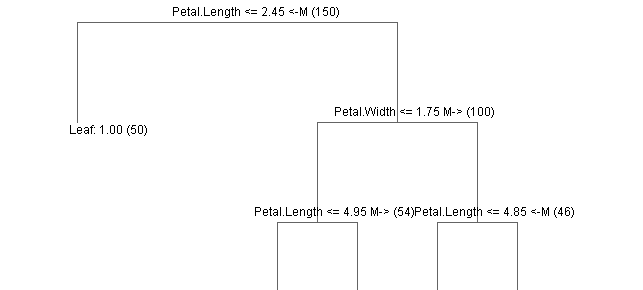
\includegraphics[width=5.3in]{classification_tree.png}
\end{figure}
\vspace{-0.3cm}
\vspace{-0.2cm}\benum\truefalsesubquestionwithpoints{14}
\vspace{-0.2cm}
\begin{enumerate}[(a)]
\item This is a regression tree model
\item This model can be written as a linear model of the form $g(\x) = b_0 + b_1 x_1 + b_2 x_2 + b_3 x_3 + b_4 x_4$ where $x_1, x_2, x_3, x_4$ are the four measurements \texttt{Sepal.Length}, \texttt{Sepal.Width}, \texttt{Petal.Length} and \texttt{Petal.Width}
\item This model is overfit
\item If the stump is considered depth zero, then this tree has a depth of 3
\item For all $\mathbb{D}$, a binary split on \texttt{Petal.Length} is the best overall split to reduce heterogeneity in the response
\item For future data, this model will likely predict setosa correctly with high probability
\item If \texttt{Petal.Length} $> 2.45$, there exists a second binary split that is able to isolate all virginica observations in one leaf and all versicolor observations in the other leaf
\item If \texttt{Petal.Length} $> 4.95$, $\hat{y}$ will always be the same
\end{enumerate}
\eenum\instr\pagebreak
%%%%%%%%%%%%%%%%%%%%%%%%%%%%%%%%%%%%%%%%%%%%%


\problem\timedsection{6} Consider the following data frame displayed in random order, where missingess is visualized in red. The last column is the response $y$ and there is no missingness in the response. The feature that has the most missingness is $x_{34}$ and the observation with the most missingness is row \#10.

\begin{figure}[htp]
\centering
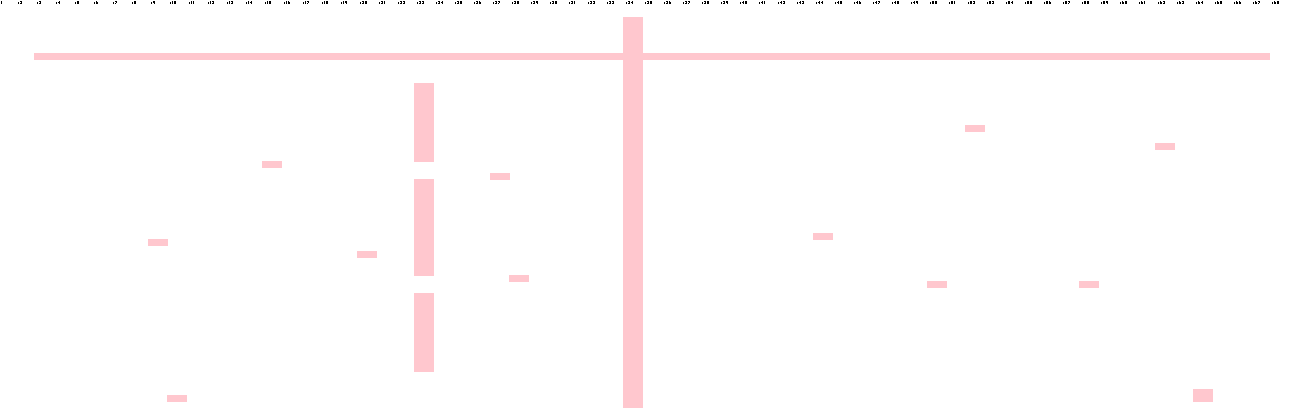
\includegraphics[width=7in]{missingness.png}
\end{figure}

\vspace{-0.2cm}\benum\truefalsesubquestionwithpoints{7}

\begin{enumerate}[(a)]
\item Dropping all observations with missingness (listwise deletion) will seriously impact future performance of any model fit with the data
\item The dataset exhibits one MCAR missingness mechanism and this mechanism is the same for all entries
\item The dataset may exhibit a different independent NMAR missingness mechanism for each feature
\item When building a predictive model, the most prudent thing to do is to drop the feature $x_{34}$ and to drop observation \#10 
\item Imputing missing values using the columns' sample averages will result in a data frame with no missingness
\item The recommended procedure is to impute with the \texttt{missForest} and then use only the imputed matrix $\X$ to construct your model ignoring the original $\X$ matrix
\end{enumerate}
\eenum\instr\pagebreak
%%%%%%%%%%%%%%%%%%%%%%%%%%%%%%%%%%%%%%%%%%%%%


\problem\timedsection{6} \ingray{Consider the following data frame, where missigness is visualized in red. The last column is the response $y$ and there is no missingness in the response. The feature that has the most missingness is $x_{34}$ and the observation with the most missingness is row \#10.}

\begin{figure}[htp]
\centering
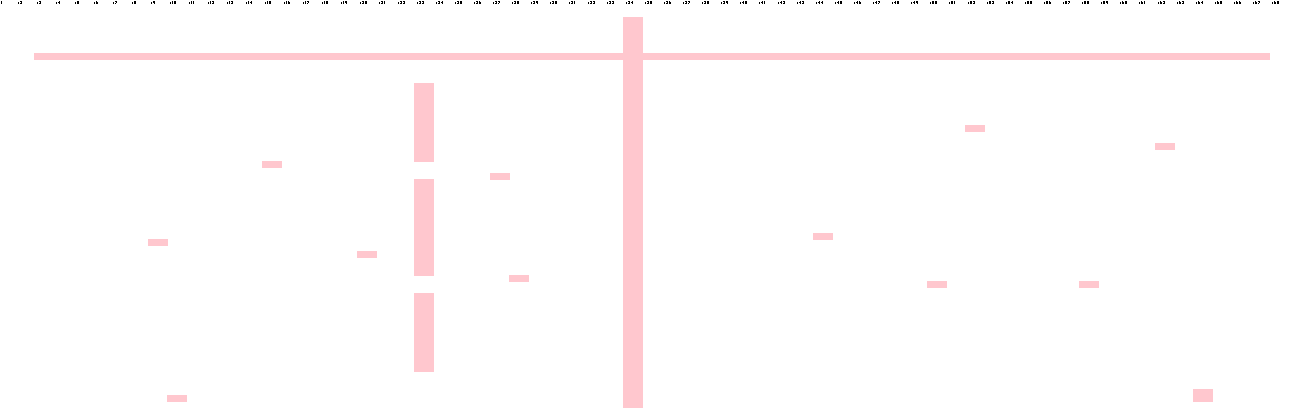
\includegraphics[width=7in]{missingness.png}
\end{figure}

\noindent Now assume that $x_{34}$ and observation \#10 were dropped and the remaining missing values were imputed via the \texttt{missForest} algorithm.

\vspace{-0.2cm}\benum\truefalsesubquestionwithpoints{6}

\begin{enumerate}[(a)]
\item An OLS model cannot be fit on the imputed data frame
\item A ridge model with $\lambda = 10^{-6}$ cannot be fit on the imputed data frame
\item A lasso model with $\lambda = 10^{-6}$ cannot be fit on the imputed data frame
\item An elastic net model with $\lambda = 10^{-6}$ and $\alpha = 0.1$ cannot be fit on the imputed data frame
\item After using the model selection procedure to select $\lambda$ for the lasso based on oos $s_e$, the number of nonzero linear coefficients in the resulting model will likely be small relative to $p$
\item After using the model selection procedure to select $\lambda$ for the ridge based on oos $s_e$, the number of nonzero linear coefficients in the resulting model will likely be small relative to $p$
\end{enumerate}
\eenum\instr\pagebreak
%%%%%%%%%%%%%%%%%%%%%%%%%%%%%%%%%%%%%%%%%%%%%

%\problem\timedsection{7} Consider the \texttt{diamonds} data frame, which has $n = 53940$ diamonds with 9 measurements each and the response variable \texttt{price} measured in USD. Below is a sample of five observations:
%
%\lstset{
%  basicstyle=\footnotesize,
%  xleftmargin=.2\textwidth, xrightmargin=.2\textwidth
%}
%\begin{lstlisting}
%  carat       cut color clarity depth table price    x    y    z
%  0.41 Very Good     D     SI2  62.3    61   638 4.72 4.75 2.95
%  0.50 Very Good     F     VS2  62.8    57  1402 5.05 5.08 3.18
%  1.03      Fair     I     SI2  65.2    56  3530 6.42 6.35 4.16
%  1.10     Ideal     I     SI1  62.1    57  5037 6.60 6.64 4.11
%  1.51 Very Good     E     VS2  63.3    61 13757 7.24 7.17 4.56
%...
%\end{lstlisting}
%\vspace{-.5cm}
%
%\noindent We wish to fit many models to this dataset: (1) OLS with the formula $y \sim .$ (2) OLS with the formula $y \sim . * .$ (3) OLS with the formula $y \sim . * . * .$ (4) a regression tree with \texttt{nodesize} = 10 (5) a Random Forest (RF) with 500 trees. The dataset is sampled into a distinct training set of size $n=3,000$, a distinct select set of $n=3,000$ and a distinct test set of $n=3,000$ and these three subsets are used in accordance with the modeling selection procedure we learned about in class.
%
%\vspace{-0.2cm}\benum\truefalsesubquestionwithpoints{14}
%
%\begin{enumerate}[(a)]
%\item The training set is fit to each of the five models above
%\item The select set is fit to each of the five models above
%\item Predicting on the training set is \qu{out of sample}
%\item Predicting on the select set is \qu{out of sample}
%\item Each of the five models above predict on the select set
%\item Each of the five models above predict on the test set
%\item The model that predicts on the test set was fit on $n=6000$ observations
%\item The final model was fit on $n=6000$ observations
%\item For the RF model, there is no need to use a separate out-of-sample set as you can assess the oos performance using the oob error estimate
%\end{enumerate}
%\eenum\instr\pagebreak
%%%%%%%%%%%%%%%%%%%%%%%%%%%%%%%%%%%%%%%%%%%%%

\problem\timedsection{14} Consider the \texttt{diamonds} data frame, which has $n = 53940$ diamonds with 9 measurements each and the response variable \texttt{price} measured in USD. We wish to fit many models to this dataset: (1) OLS with the formula $y \sim .$ (2) OLS with the formula $y \sim . * .$ (3) OLS with the formula $y \sim . * . * .$ (4) a regression tree with \texttt{nodesize} = 10 (5) a Random Forest (RF) with 500 trees. Consider two model selection procedures:
\vspace{-0.1cm}
\begin{enumerate}[A.]
\item The three-split dataset model selection procedure where the original dataset is sampled into a distinct training set of size $n=3,000$, a distinct select set of $n=3,000$ and a distinct test set of $n=3,000$.
\item The \textit{nested resampling procedure} for model selection where $K_{select} = 3$ and $K_{test} = 5$ on a subset of $n=9,000$ observations from the original data frame.
\end{enumerate}

\vspace{-0.2cm}\benum\truefalsesubquestionwithpoints{16}

\begin{enumerate}[(a)]
\item In procedure [A], the training set is fit to each of the five models above
\item In procedure [A], the the select set is fit to each of the five models above
\item In procedure [A], predicting on the training set is \qu{out of sample}
\item In procedure [A], predicting on the select set is \qu{out of sample}
\item In procedure [A], each of the five models above predict on the test set
\item In procedure [A], the model that predicts on the test set was fit on $n=6000$ observations
\item In procedure [A], the final model was fit on $n=6000$ observations
%\item For the RF model, there is no need to use a separate out-of-sample set as you can assess the oos performance using the oob error estimate
\item Procedure [B] is more computationally costly than procedure [A]
\item Procedure [B] has lower variance in its estimate of future performance
\item Procedure [B] is likely to select a model with better future performance than procedure [A]
\item There are a total of 16 models fit during procedure [B] including the final model
\item There are a total of 26 models fit during procedure [B] including the final model
\item There are a total of 65 models fit during procedure [B] including the final model
\item There are a total of 76 models fit during procedure [B] including the final model
\item During procedure [B], for each of the $K_{test}$ outer resamplings, there could be a different model that predicts on the test set
\item In procedure [B], the final model will be the modal model out of the $K_{test}$ models selected
\end{enumerate}
\eenum\instr\pagebreak
%%%%%%%%%%%%%%%%%%%%%%%%%%%%%%%%%%%%%%%%%%%%%


\problem\timedsection{8} \ingray{Consider the \texttt{diamonds} data frame, which has $n = 53940$ diamonds with 9 measurements each and the response variable \texttt{price} measured in USD.} Beginning with the design matrix $\tilde{\X}$ created by the OLS model of $y \sim . * . * .$ we consider the \emph{greedy forward stepwise} linear model algorithm. The dataset is sampled into a distinct training set of size $n=3,000$, a distinct select set of $n=3,000$ and a distinct test set of $n=3,000$ and these three subsets are used in accordance with the modeling selection procedure we learned about in class.

\vspace{-0.2cm}\benum\truefalsesubquestionwithpoints{7}

\begin{enumerate}[(a)]
\item This algorithm at most has $p+1$ iterations where $p+1$ is the number of columns in $\tilde{\X}$ and in each iteration, it fits a different linear model
\item This algorithm likely has less than $p+1$ iterations
\item The prediction error in the training set is monotonically decreasing
\item The prediction error in the select set is monotonically decreasing
\item The prediction error in the test set is monotonically decreasing
\item When predicting on the test set, the model will definitely have the same number of degrees of freedom as the final model
\item The future performance of the model selected by the \emph{greedy forward stepwise} linear model algorithm will be better than the future performance of the OLS model of  $y \sim .$ based on your knowledge of this dataset from class
\end{enumerate}
\eenum\instr\pagebreak
%%%%%%%%%%%%%%%%%%%%%%%%%%%%%%%%%%%%%%%%%%%%%


\problem\timedsection{7} \ingray{Consider the \texttt{diamonds} data frame, which has $n = 53,940$ diamonds with 9 measurements each and the response variable \texttt{price} measured in USD. Beginning with the design matrix $\tilde{\X}$ created by the OLS model of $y \sim . * . * .$ we consider the \emph{greedy forward stepwise} linear model algorithm. The dataset is sampled into a distinct training set of size $n=3,000$, a distinct select set of $n=3,000$ and a distinct test set of $n=3,000$ and these three subsets are used in accordance with the modeling selection procedure we learned about in class.} The design matrix $\tilde{\X}$ has $p+1 = 1477$ number of columns. Consider the case where we run through all of the $t = 1, 2, \ldots, 1477$ iterations of this stepwise algorithm.

\vspace{-0.2cm}\benum\truefalsesubquestionwithpoints{7}

Let $g_t$ denote the model fit at every iteration $t$.

\begin{enumerate}[(a)]
\item As $t$ increases the bias of $g_t$ increases monotonically
\item As $t$ increases the variance of $g_t$ increases monotonically
\item As $t$ increases the MSE of $g_t$ increases monotonically 
\item $g_1, g_2, \ldots, g_{1477}$ are independent models\\

Consider the model $g_{avg}$ that averages models $g_1, g_2, \ldots, g_{1477}$.

\item $g_{avg}$ is called a \qu{bagged} model
\item $g_{avg}$ has lower bias than $g_{1477}$
\item $g_{avg}$ always has lower MSE than the model that was selected by the greedy forward stepwise linear model algorithm
\end{enumerate}
\eenum\instr\pagebreak
%%%%%%%%%%%%%%%%%%%%%%%%%%%%%%%%%%%%%%%%%%%%%


\problem\timedsection{12} Consider the \texttt{adult} data frame, which has data on $n = 32,560$ people with 14 measurements each and the response variable \texttt{income} which is binary (1 = the person has an income $>$50K and 0 = the person has an income  $\leq$50K). Consider the following model fit to \texttt{adult\_train}, a training set of $n=10,000$ leaving the remainder of the data as a holdout set. The $\b$ vector for the fitted model is displayed below on the last line.

\lstset{
  basicstyle=\footnotesize,
  xleftmargin=.0\textwidth, xrightmargin=.0\textwidth
}
\begin{lstlisting}
> lmod = glm(income ~ age + hours_per_week + capital_gain + education_num, adult_train, family = "binomial")
Warning message:
glm.fit: fitted probabilities numerically 0 or 1 occurred 
> coef(lmod)
   (Intercept)            age hours_per_week   capital_gain  education_num 
       -8.1582         0.0454         0.0380         0.0003         0.3200
\end{lstlisting}

\vspace{-0.8cm}\benum\truefalsesubquestionwithpoints{12}

\begin{enumerate}[(a)]
\item The vector $\b$ was computed solely using linear algebra calculations
\item For a future person $\x_*$, the quantity $\x_*\b$ can be used to produce probability predictions in the set (0, 1)
\item For a future person $\x_*$, if $\x_*\b < 0$, this model is predicting that it is impossible for this person's income to be $>$50K
\item The Brier score for this model's predictions in-sample will likely be closer to zero than the Brier score for predictions out-of-sample.
\item The probability predictions of this model will be the same predictions as a probit model fit to the same data
\item \qu{For a future person $\x_*$, the probability that this person's income $>$50K will increase by 0.044 if the person becomes one year older}.
\item \qu{For a future person $\x_*$, the probability that this person's income $>$50K will increase by 0.044 if the person becomes one year older as long as the three other measurements for this person do not change}.
\item If \texttt{age} increases and the three other variables remain the same, the predicted probability will increase for any $\x$
\item The warning message means there was numerical underflow and/or overflow during the computation of $\b$
\item For a 20yr-old with no job, capital gains or education, the probability he has an income of $>$50K is 0.9993 to the nearest four significant digits
\item For a 20yr-old with no job, capital gains or education, the probability he has an income of $>$50K is 0.0007095 to the nearest four significant digits
\item You have all the information necessary in this problem statement to trace out a DET curve
\end{enumerate}
\eenum\instr\pagebreak
%%%%%%%%%%%%%%%%%%%%%%%%%%%%%%%%%%%%%%%%%%%%%

\problem\timedsection{14} \ingray{Consider the \texttt{adult} data frame, which has data on $n = 32,560$ people with 14 measurements each and the response variable \texttt{income} which is binary (1 = the person has an income $>$50K and 0 = the person has an income  $\leq$50K).} Considering the model from the previous quesiton fit to \texttt{adult\_train}, a training set of $n=10,000$ leaving the remainder of the data as a holdout set, we now predict on \texttt{adult\_test} and perform binary classification:

\lstset{
  basicstyle=\footnotesize,
  xleftmargin=.15\textwidth, xrightmargin=.15\textwidth
}
\begin{lstlisting}
> yhat = as.numeric(predict(lmod, adult_test, type = "response") > 0.9)
> table(y_test, yhat)
             yhat
y_test     0     1
     0 15107    30
     1  4439   585
\end{lstlisting}

\vspace{-0.8cm}\benum\truefalsesubquestionwithpoints{9}

\begin{enumerate}[(a)]
\item This is likely an asymmetric cost classification model
\item The FDR, FOR, FPR calculated using the above table are honest estimates of future performance
\item This model makes mistakes 22.2\% of the time to the nearest three significant digits
\item This classification model is absolutely the best classification model you could build from \texttt{lmod} to minimize costs when the cost of a FP is \$9 and the cost of a FN is \$9
\item This model implies the point (0.00198, 0.116) on an ROC curve to the nearest three significant digits
\item When predicting in the future using this classification model, if $\hat{y} = 1$, then the probability of making an error is 4.88\% to the nearest three signification digits
\item If the cost of a false positive is \$100 and the cost of false negatives was negligible and there is no reward for classifying correctly, then you expect to lose \$0.15 per prediction to the nearest two signification digits
\item If the probability threshold was increased within the binary classification model, then the number of FP's would decrease
\item You have all the information necessary in this problem statement to compute the AUC for \texttt{lmod}
\end{enumerate}
\eenum\instr\pagebreak
%%%%%%%%%%%%%%%%%%%%%%%%%%%%%%%%%%%%%%%%%%%%%

\end{document}
%%%%%%%%%%%%%%%%%%%%%%%%%%%%%%%%%%%%%%%%%%%%%
%%%%%%%%%%%%%%%%%%%%%%%%%%%%%%%%%%%%%%%%%%%%%
%%%%%%%%%%%%%%%%%%%%%%%%%%%%%%%%%%%%%%%%%%%%%
%%%%%%%%%%%%%%%%%%%%%%%%%%%%%%%%%%%%%%%%%%%%%
%%%%%%%%%%%%%%%%%%%%%%%%%%%%%%%%%%%%%%%%%%%%%
%%%%%%%%%%%%%%%%%%%%%%%%%%%%%%%%%%%%%%%%%%%%%
%%%%%%%%%%%%%%%%%%%%%%%%%%%%%%%%%%%%%%%%%%%%%
%%%%%%%%%%%%%%%%%%%%%%%%%%%%%%%%%%%%%%%%%%%%%
%%%%%%%%%%%%%%%%%%%%%%%%%%%%%%%%%%%%%%%%%%%%%
%%%%%%%%%%%%%%%%%%%%%%%%%%%%%%%%%%%%%%%%%%%%%
%%%%%%%%%%%%%%%%%%%%%%%%%%%%%%%%%%%%%%%%%%%%%
%%%%%%%%%%%%%%%%%%%%%%%%%%%%%%%%%%%%%%%%%%%%%
%%%%%%%%%%%%%%%%%%%%%%%%%%%%%%%%%%%%%%%%%%%%%















